\documentclass[12pt]{extarticle}
\usepackage[letterpaper,top=20mm,bottom=20mm,left=16mm,right=16mm,headheight=16pt,headsep=7mm,footskip=10mm]{geometry}
\usepackage[T1]{fontenc}
\usepackage{tgheros}
\renewcommand{\familydefault}{\sfdefault}
\usepackage{tikz}
\usetikzlibrary{arrows.meta,decorations.pathreplacing}
\usepackage{fancyhdr}
\usepackage{xcolor}
\definecolor{cardred}{RGB}{206,38,38}
\definecolor{cardblue}{RGB}{28,92,196}
\colorlet{stripred}{cardred!32}
\colorlet{stripblue}{cardblue!28}
\colorlet{panelgrey}{black!20}
\colorlet{boxgrey}{black!45}
\tikzset{cardedge/.style={draw=black!70,line width=0.5pt}}
\pagestyle{fancy}
\fancyhf{}
\fancyhead[L]{\small Week 58 / Fair division / Grades 2--3}
\fancyfoot[L]{\small Bellingham Math Circle / Week 58 / W58-RV-M-v1}
\fancyfoot[R]{\small \thepage}
\renewcommand{\headrulewidth}{0.4pt}
\renewcommand{\footrulewidth}{0pt}
\setlength{\parindent}{0pt}
\setlength{\parskip}{4pt}
\newcommand{\prob}[1]{\par\noindent\textbf{Problem #1:} }
\begin{document}
A train is a row of goods cards. To share a train, cut it at some of the gaps between neighbouring cards, so that every card stays whole, and put each piece into one of two trays. A tray may get more than one piece. Both trays must get the same number of red cards and the same number of blue cards.
\begin{center}
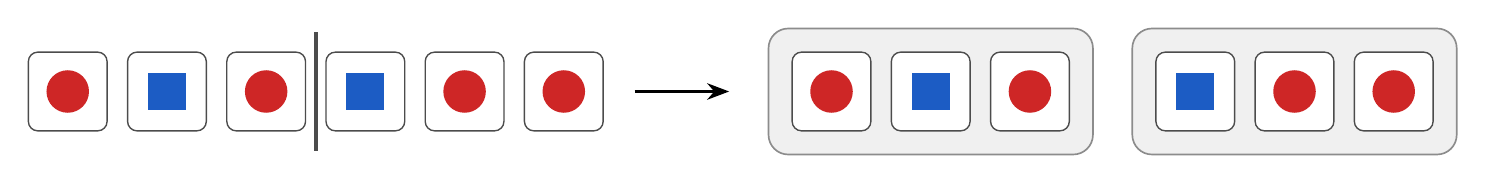
\begin{tikzpicture}[x=1mm,y=1mm]
\draw[cardedge, fill=white, rounded corners=1.2mm] (0,0) rectangle (10,10);
\fill[cardred] (5,5) circle (2.7mm);
\draw[cardedge, fill=white, rounded corners=1.2mm] (12.6,0) rectangle (22.6,10);
\fill[cardblue] (15.2,2.6) rectangle (20,7.4);
\draw[cardedge, fill=white, rounded corners=1.2mm] (25.2,0) rectangle (35.2,10);
\fill[cardred] (30.2,5) circle (2.7mm);
\draw[cardedge, fill=white, rounded corners=1.2mm] (37.8,0) rectangle (47.8,10);
\fill[cardblue] (40.4,2.6) rectangle (45.2,7.4);
\draw[cardedge, fill=white, rounded corners=1.2mm] (50.4,0) rectangle (60.4,10);
\fill[cardred] (55.4,5) circle (2.7mm);
\draw[cardedge, fill=white, rounded corners=1.2mm] (63,0) rectangle (73,10);
\fill[cardred] (68,5) circle (2.7mm);
\draw[black!70, line width=1.4pt] (36.5,-2.5) -- (36.5,12.5);
\draw[-{Stealth[length=2.8mm]}, line width=0.9pt] (77,5) -- (89,5);
\draw[black!45, fill=black!6, line width=0.6pt, rounded corners=2.5mm] (94,-3) rectangle (135.2,13);
\draw[cardedge, fill=white, rounded corners=1.2mm] (97,0) rectangle (107,10);
\fill[cardred] (102,5) circle (2.7mm);
\draw[cardedge, fill=white, rounded corners=1.2mm] (109.6,0) rectangle (119.6,10);
\fill[cardblue] (112.2,2.6) rectangle (117,7.4);
\draw[cardedge, fill=white, rounded corners=1.2mm] (122.2,0) rectangle (132.2,10);
\fill[cardred] (127.2,5) circle (2.7mm);
\draw[black!45, fill=black!6, line width=0.6pt, rounded corners=2.5mm] (140.2,-3) rectangle (181.4,13);
\draw[cardedge, fill=white, rounded corners=1.2mm] (143.2,0) rectangle (153.2,10);
\fill[cardblue] (145.8,2.6) rectangle (150.6,7.4);
\draw[cardedge, fill=white, rounded corners=1.2mm] (155.8,0) rectangle (165.8,10);
\fill[cardred] (160.8,5) circle (2.7mm);
\draw[cardedge, fill=white, rounded corners=1.2mm] (168.4,0) rectangle (178.4,10);
\fill[cardred] (173.4,5) circle (2.7mm);
\end{tikzpicture}
\end{center}
\vspace{1mm}
\prob{1}Find every train you can make with two red cards and two blue cards, counting only the order of the colours. Share each one with as few cuts as you can.
\vspace{4mm}
\begin{center}
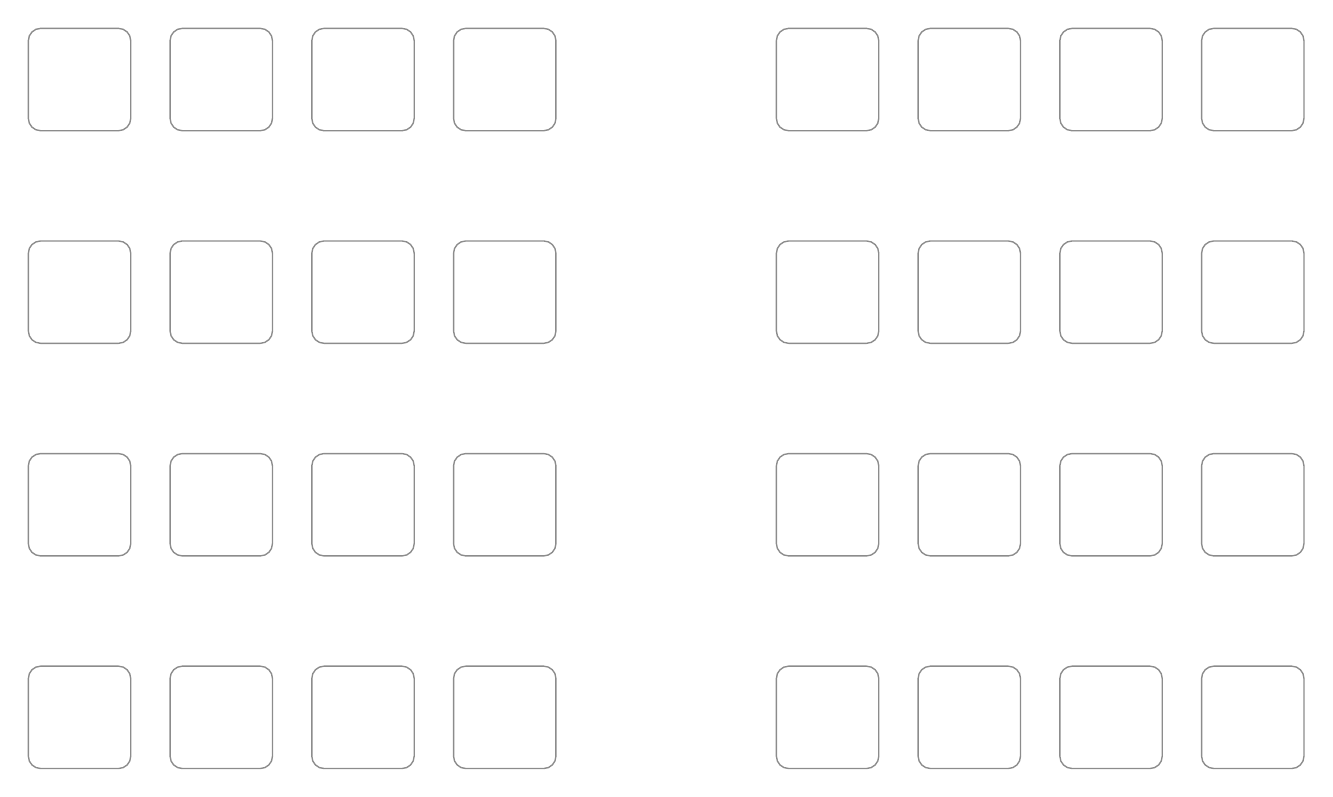
\begin{tikzpicture}[x=1mm,y=1mm]
\draw[boxgrey, line width=0.5pt, rounded corners=1.56mm] (0,0) rectangle (13,13);
\draw[boxgrey, line width=0.5pt, rounded corners=1.56mm] (18,0) rectangle (31,13);
\draw[boxgrey, line width=0.5pt, rounded corners=1.56mm] (36,0) rectangle (49,13);
\draw[boxgrey, line width=0.5pt, rounded corners=1.56mm] (54,0) rectangle (67,13);
\draw[boxgrey, line width=0.5pt, rounded corners=1.56mm] (95,0) rectangle (108,13);
\draw[boxgrey, line width=0.5pt, rounded corners=1.56mm] (113,0) rectangle (126,13);
\draw[boxgrey, line width=0.5pt, rounded corners=1.56mm] (131,0) rectangle (144,13);
\draw[boxgrey, line width=0.5pt, rounded corners=1.56mm] (149,0) rectangle (162,13);
\draw[boxgrey, line width=0.5pt, rounded corners=1.56mm] (0,-27) rectangle (13,-14);
\draw[boxgrey, line width=0.5pt, rounded corners=1.56mm] (18,-27) rectangle (31,-14);
\draw[boxgrey, line width=0.5pt, rounded corners=1.56mm] (36,-27) rectangle (49,-14);
\draw[boxgrey, line width=0.5pt, rounded corners=1.56mm] (54,-27) rectangle (67,-14);
\draw[boxgrey, line width=0.5pt, rounded corners=1.56mm] (95,-27) rectangle (108,-14);
\draw[boxgrey, line width=0.5pt, rounded corners=1.56mm] (113,-27) rectangle (126,-14);
\draw[boxgrey, line width=0.5pt, rounded corners=1.56mm] (131,-27) rectangle (144,-14);
\draw[boxgrey, line width=0.5pt, rounded corners=1.56mm] (149,-27) rectangle (162,-14);
\draw[boxgrey, line width=0.5pt, rounded corners=1.56mm] (0,-54) rectangle (13,-41);
\draw[boxgrey, line width=0.5pt, rounded corners=1.56mm] (18,-54) rectangle (31,-41);
\draw[boxgrey, line width=0.5pt, rounded corners=1.56mm] (36,-54) rectangle (49,-41);
\draw[boxgrey, line width=0.5pt, rounded corners=1.56mm] (54,-54) rectangle (67,-41);
\draw[boxgrey, line width=0.5pt, rounded corners=1.56mm] (95,-54) rectangle (108,-41);
\draw[boxgrey, line width=0.5pt, rounded corners=1.56mm] (113,-54) rectangle (126,-41);
\draw[boxgrey, line width=0.5pt, rounded corners=1.56mm] (131,-54) rectangle (144,-41);
\draw[boxgrey, line width=0.5pt, rounded corners=1.56mm] (149,-54) rectangle (162,-41);
\draw[boxgrey, line width=0.5pt, rounded corners=1.56mm] (0,-81) rectangle (13,-68);
\draw[boxgrey, line width=0.5pt, rounded corners=1.56mm] (18,-81) rectangle (31,-68);
\draw[boxgrey, line width=0.5pt, rounded corners=1.56mm] (36,-81) rectangle (49,-68);
\draw[boxgrey, line width=0.5pt, rounded corners=1.56mm] (54,-81) rectangle (67,-68);
\draw[boxgrey, line width=0.5pt, rounded corners=1.56mm] (95,-81) rectangle (108,-68);
\draw[boxgrey, line width=0.5pt, rounded corners=1.56mm] (113,-81) rectangle (126,-68);
\draw[boxgrey, line width=0.5pt, rounded corners=1.56mm] (131,-81) rectangle (144,-68);
\draw[boxgrey, line width=0.5pt, rounded corners=1.56mm] (149,-81) rectangle (162,-68);
\end{tikzpicture}
\end{center}
\newpage
\prob{2}Share each of these trains with as few cuts as you can. If a train cannot be shared, cross it out.
\vspace{4mm}
\begin{center}
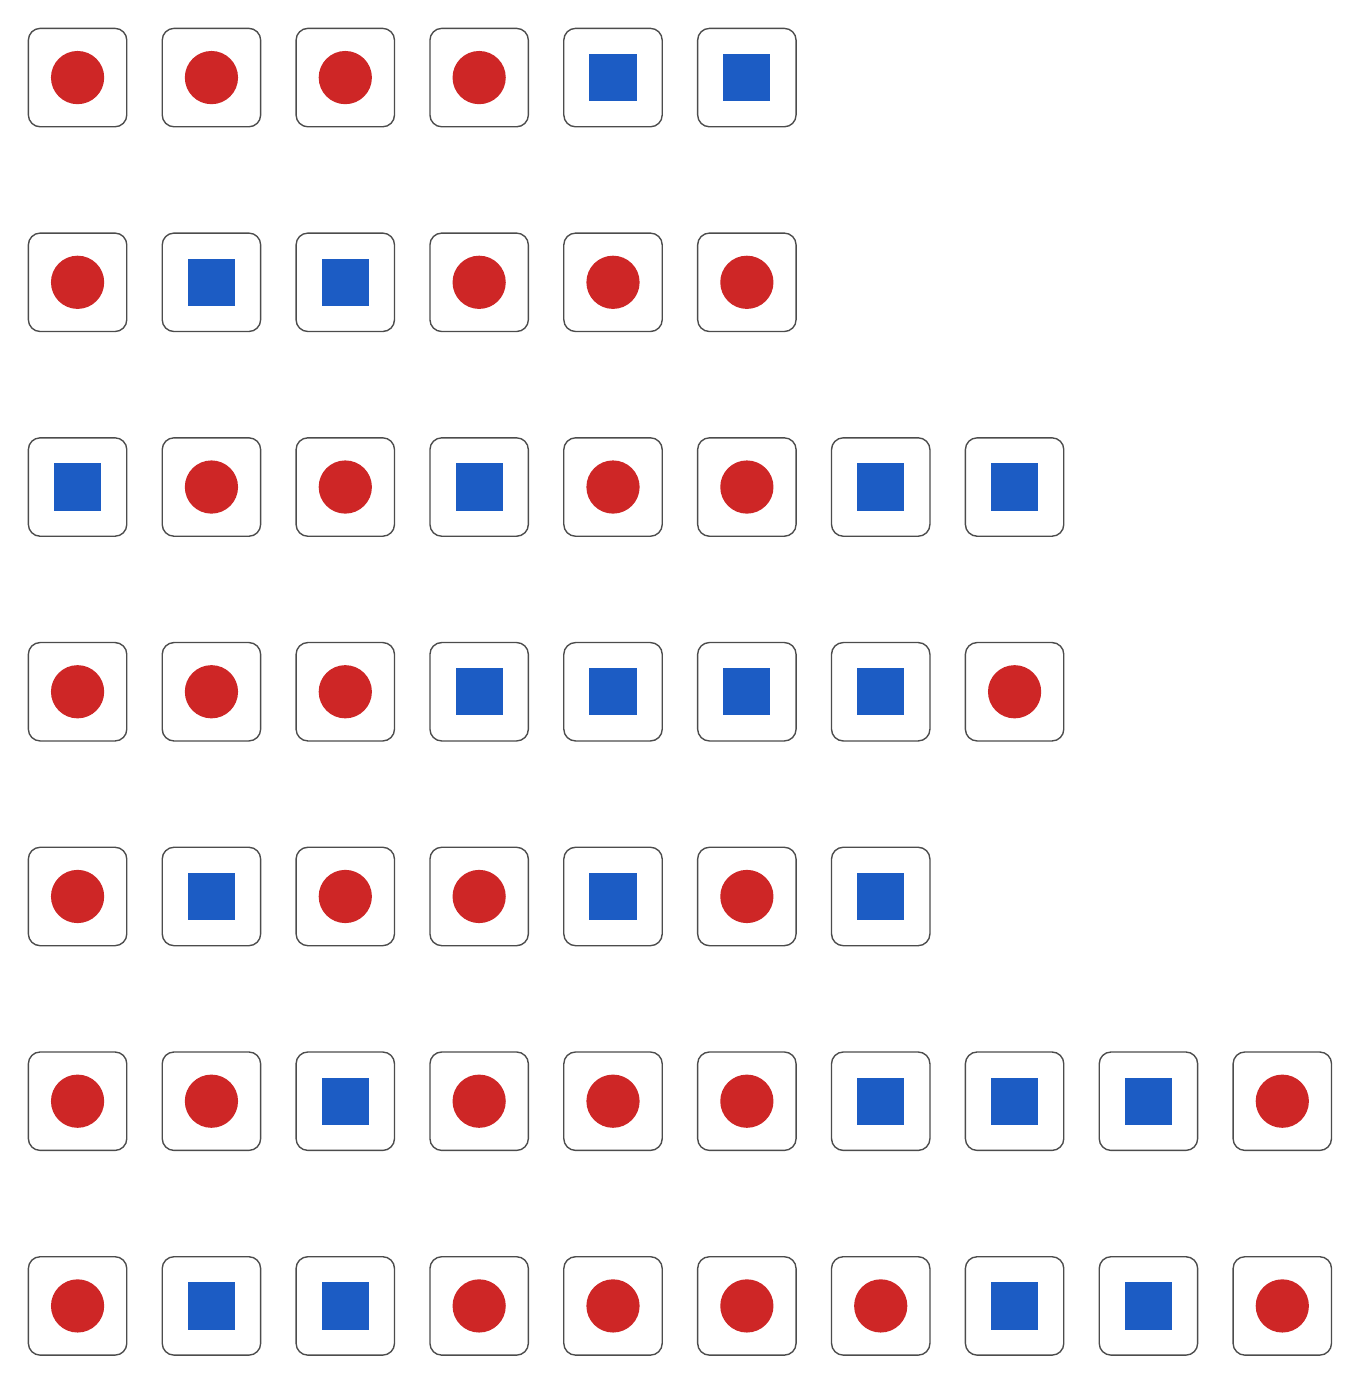
\begin{tikzpicture}[x=1mm,y=1mm]
\draw[cardedge, fill=white, rounded corners=1.5mm] (0,0) rectangle (12.5,12.5);
\fill[cardred] (6.25,6.25) circle (3.38mm);
\draw[cardedge, fill=white, rounded corners=1.5mm] (17,0) rectangle (29.5,12.5);
\fill[cardred] (23.25,6.25) circle (3.38mm);
\draw[cardedge, fill=white, rounded corners=1.5mm] (34,0) rectangle (46.5,12.5);
\fill[cardred] (40.25,6.25) circle (3.38mm);
\draw[cardedge, fill=white, rounded corners=1.5mm] (51,0) rectangle (63.5,12.5);
\fill[cardred] (57.25,6.25) circle (3.38mm);
\draw[cardedge, fill=white, rounded corners=1.5mm] (68,0) rectangle (80.5,12.5);
\fill[cardblue] (71.25,3.25) rectangle (77.25,9.25);
\draw[cardedge, fill=white, rounded corners=1.5mm] (85,0) rectangle (97.5,12.5);
\fill[cardblue] (88.25,3.25) rectangle (94.25,9.25);
\draw[cardedge, fill=white, rounded corners=1.5mm] (0,-26) rectangle (12.5,-13.5);
\fill[cardred] (6.25,-19.75) circle (3.38mm);
\draw[cardedge, fill=white, rounded corners=1.5mm] (17,-26) rectangle (29.5,-13.5);
\fill[cardblue] (20.25,-22.75) rectangle (26.25,-16.75);
\draw[cardedge, fill=white, rounded corners=1.5mm] (34,-26) rectangle (46.5,-13.5);
\fill[cardblue] (37.25,-22.75) rectangle (43.25,-16.75);
\draw[cardedge, fill=white, rounded corners=1.5mm] (51,-26) rectangle (63.5,-13.5);
\fill[cardred] (57.25,-19.75) circle (3.38mm);
\draw[cardedge, fill=white, rounded corners=1.5mm] (68,-26) rectangle (80.5,-13.5);
\fill[cardred] (74.25,-19.75) circle (3.38mm);
\draw[cardedge, fill=white, rounded corners=1.5mm] (85,-26) rectangle (97.5,-13.5);
\fill[cardred] (91.25,-19.75) circle (3.38mm);
\draw[cardedge, fill=white, rounded corners=1.5mm] (0,-52) rectangle (12.5,-39.5);
\fill[cardblue] (3.25,-48.75) rectangle (9.25,-42.75);
\draw[cardedge, fill=white, rounded corners=1.5mm] (17,-52) rectangle (29.5,-39.5);
\fill[cardred] (23.25,-45.75) circle (3.38mm);
\draw[cardedge, fill=white, rounded corners=1.5mm] (34,-52) rectangle (46.5,-39.5);
\fill[cardred] (40.25,-45.75) circle (3.38mm);
\draw[cardedge, fill=white, rounded corners=1.5mm] (51,-52) rectangle (63.5,-39.5);
\fill[cardblue] (54.25,-48.75) rectangle (60.25,-42.75);
\draw[cardedge, fill=white, rounded corners=1.5mm] (68,-52) rectangle (80.5,-39.5);
\fill[cardred] (74.25,-45.75) circle (3.38mm);
\draw[cardedge, fill=white, rounded corners=1.5mm] (85,-52) rectangle (97.5,-39.5);
\fill[cardred] (91.25,-45.75) circle (3.38mm);
\draw[cardedge, fill=white, rounded corners=1.5mm] (102,-52) rectangle (114.5,-39.5);
\fill[cardblue] (105.25,-48.75) rectangle (111.25,-42.75);
\draw[cardedge, fill=white, rounded corners=1.5mm] (119,-52) rectangle (131.5,-39.5);
\fill[cardblue] (122.25,-48.75) rectangle (128.25,-42.75);
\draw[cardedge, fill=white, rounded corners=1.5mm] (0,-78) rectangle (12.5,-65.5);
\fill[cardred] (6.25,-71.75) circle (3.38mm);
\draw[cardedge, fill=white, rounded corners=1.5mm] (17,-78) rectangle (29.5,-65.5);
\fill[cardred] (23.25,-71.75) circle (3.38mm);
\draw[cardedge, fill=white, rounded corners=1.5mm] (34,-78) rectangle (46.5,-65.5);
\fill[cardred] (40.25,-71.75) circle (3.38mm);
\draw[cardedge, fill=white, rounded corners=1.5mm] (51,-78) rectangle (63.5,-65.5);
\fill[cardblue] (54.25,-74.75) rectangle (60.25,-68.75);
\draw[cardedge, fill=white, rounded corners=1.5mm] (68,-78) rectangle (80.5,-65.5);
\fill[cardblue] (71.25,-74.75) rectangle (77.25,-68.75);
\draw[cardedge, fill=white, rounded corners=1.5mm] (85,-78) rectangle (97.5,-65.5);
\fill[cardblue] (88.25,-74.75) rectangle (94.25,-68.75);
\draw[cardedge, fill=white, rounded corners=1.5mm] (102,-78) rectangle (114.5,-65.5);
\fill[cardblue] (105.25,-74.75) rectangle (111.25,-68.75);
\draw[cardedge, fill=white, rounded corners=1.5mm] (119,-78) rectangle (131.5,-65.5);
\fill[cardred] (125.25,-71.75) circle (3.38mm);
\draw[cardedge, fill=white, rounded corners=1.5mm] (0,-104) rectangle (12.5,-91.5);
\fill[cardred] (6.25,-97.75) circle (3.38mm);
\draw[cardedge, fill=white, rounded corners=1.5mm] (17,-104) rectangle (29.5,-91.5);
\fill[cardblue] (20.25,-100.75) rectangle (26.25,-94.75);
\draw[cardedge, fill=white, rounded corners=1.5mm] (34,-104) rectangle (46.5,-91.5);
\fill[cardred] (40.25,-97.75) circle (3.38mm);
\draw[cardedge, fill=white, rounded corners=1.5mm] (51,-104) rectangle (63.5,-91.5);
\fill[cardred] (57.25,-97.75) circle (3.38mm);
\draw[cardedge, fill=white, rounded corners=1.5mm] (68,-104) rectangle (80.5,-91.5);
\fill[cardblue] (71.25,-100.75) rectangle (77.25,-94.75);
\draw[cardedge, fill=white, rounded corners=1.5mm] (85,-104) rectangle (97.5,-91.5);
\fill[cardred] (91.25,-97.75) circle (3.38mm);
\draw[cardedge, fill=white, rounded corners=1.5mm] (102,-104) rectangle (114.5,-91.5);
\fill[cardblue] (105.25,-100.75) rectangle (111.25,-94.75);
\draw[cardedge, fill=white, rounded corners=1.5mm] (0,-130) rectangle (12.5,-117.5);
\fill[cardred] (6.25,-123.75) circle (3.38mm);
\draw[cardedge, fill=white, rounded corners=1.5mm] (17,-130) rectangle (29.5,-117.5);
\fill[cardred] (23.25,-123.75) circle (3.38mm);
\draw[cardedge, fill=white, rounded corners=1.5mm] (34,-130) rectangle (46.5,-117.5);
\fill[cardblue] (37.25,-126.75) rectangle (43.25,-120.75);
\draw[cardedge, fill=white, rounded corners=1.5mm] (51,-130) rectangle (63.5,-117.5);
\fill[cardred] (57.25,-123.75) circle (3.38mm);
\draw[cardedge, fill=white, rounded corners=1.5mm] (68,-130) rectangle (80.5,-117.5);
\fill[cardred] (74.25,-123.75) circle (3.38mm);
\draw[cardedge, fill=white, rounded corners=1.5mm] (85,-130) rectangle (97.5,-117.5);
\fill[cardred] (91.25,-123.75) circle (3.38mm);
\draw[cardedge, fill=white, rounded corners=1.5mm] (102,-130) rectangle (114.5,-117.5);
\fill[cardblue] (105.25,-126.75) rectangle (111.25,-120.75);
\draw[cardedge, fill=white, rounded corners=1.5mm] (119,-130) rectangle (131.5,-117.5);
\fill[cardblue] (122.25,-126.75) rectangle (128.25,-120.75);
\draw[cardedge, fill=white, rounded corners=1.5mm] (136,-130) rectangle (148.5,-117.5);
\fill[cardblue] (139.25,-126.75) rectangle (145.25,-120.75);
\draw[cardedge, fill=white, rounded corners=1.5mm] (153,-130) rectangle (165.5,-117.5);
\fill[cardred] (159.25,-123.75) circle (3.38mm);
\draw[cardedge, fill=white, rounded corners=1.5mm] (0,-156) rectangle (12.5,-143.5);
\fill[cardred] (6.25,-149.75) circle (3.38mm);
\draw[cardedge, fill=white, rounded corners=1.5mm] (17,-156) rectangle (29.5,-143.5);
\fill[cardblue] (20.25,-152.75) rectangle (26.25,-146.75);
\draw[cardedge, fill=white, rounded corners=1.5mm] (34,-156) rectangle (46.5,-143.5);
\fill[cardblue] (37.25,-152.75) rectangle (43.25,-146.75);
\draw[cardedge, fill=white, rounded corners=1.5mm] (51,-156) rectangle (63.5,-143.5);
\fill[cardred] (57.25,-149.75) circle (3.38mm);
\draw[cardedge, fill=white, rounded corners=1.5mm] (68,-156) rectangle (80.5,-143.5);
\fill[cardred] (74.25,-149.75) circle (3.38mm);
\draw[cardedge, fill=white, rounded corners=1.5mm] (85,-156) rectangle (97.5,-143.5);
\fill[cardred] (91.25,-149.75) circle (3.38mm);
\draw[cardedge, fill=white, rounded corners=1.5mm] (102,-156) rectangle (114.5,-143.5);
\fill[cardred] (108.25,-149.75) circle (3.38mm);
\draw[cardedge, fill=white, rounded corners=1.5mm] (119,-156) rectangle (131.5,-143.5);
\fill[cardblue] (122.25,-152.75) rectangle (128.25,-146.75);
\draw[cardedge, fill=white, rounded corners=1.5mm] (136,-156) rectangle (148.5,-143.5);
\fill[cardblue] (139.25,-152.75) rectangle (145.25,-146.75);
\draw[cardedge, fill=white, rounded corners=1.5mm] (153,-156) rectangle (165.5,-143.5);
\fill[cardred] (159.25,-149.75) circle (3.38mm);
\path (0,0) -- (165.5,0);
\end{tikzpicture}
\end{center}
\newpage
\prob{3}One person uses the two-person card A, and another person uses the two-person card B.
\begin{center}
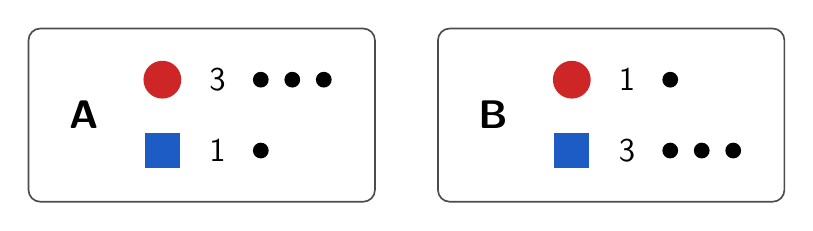
\begin{tikzpicture}[x=1mm,y=1mm]
\draw[black!70, line width=0.6pt, rounded corners=1.5mm] (0,0) rectangle (44,22);
\node[font=\Large\bfseries] at (7,11) {A};
\fill[cardred] (17,15.5) circle (2.4mm);
\node[font=\large] at (24,15.5) {3};
\fill[black] (29.5,15.5) circle (1mm);
\fill[black] (33.5,15.5) circle (1mm);
\fill[black] (37.5,15.5) circle (1mm);
\fill[cardblue] (14.8,4.3) rectangle (19.2,8.7);
\node[font=\large] at (24,6.5) {1};
\fill[black] (29.5,6.5) circle (1mm);
\draw[black!70, line width=0.6pt, rounded corners=1.5mm] (52,0) rectangle (96,22);
\node[font=\Large\bfseries] at (59,11) {B};
\fill[cardred] (69,15.5) circle (2.4mm);
\node[font=\large] at (76,15.5) {1};
\fill[black] (81.5,15.5) circle (1mm);
\fill[cardblue] (66.8,4.3) rectangle (71.2,8.7);
\node[font=\large] at (76,6.5) {3};
\fill[black] (81.5,6.5) circle (1mm);
\fill[black] (85.5,6.5) circle (1mm);
\fill[black] (89.5,6.5) circle (1mm);
\end{tikzpicture}
\end{center}
On a strip, each number is the value of the whole 120\,mm panel of that colour, and value follows length: 40\,mm of red is worth 1 to A. Every cut goes straight across the strip. Share one strip between two trays so that A finds the two trays worth the same, and B also finds them worth the same. Use as few cuts as you can. Can one cut do it? Measure on your strip from the red end, and mark in pencil before anyone cuts.
\vspace{6mm}
\begin{center}
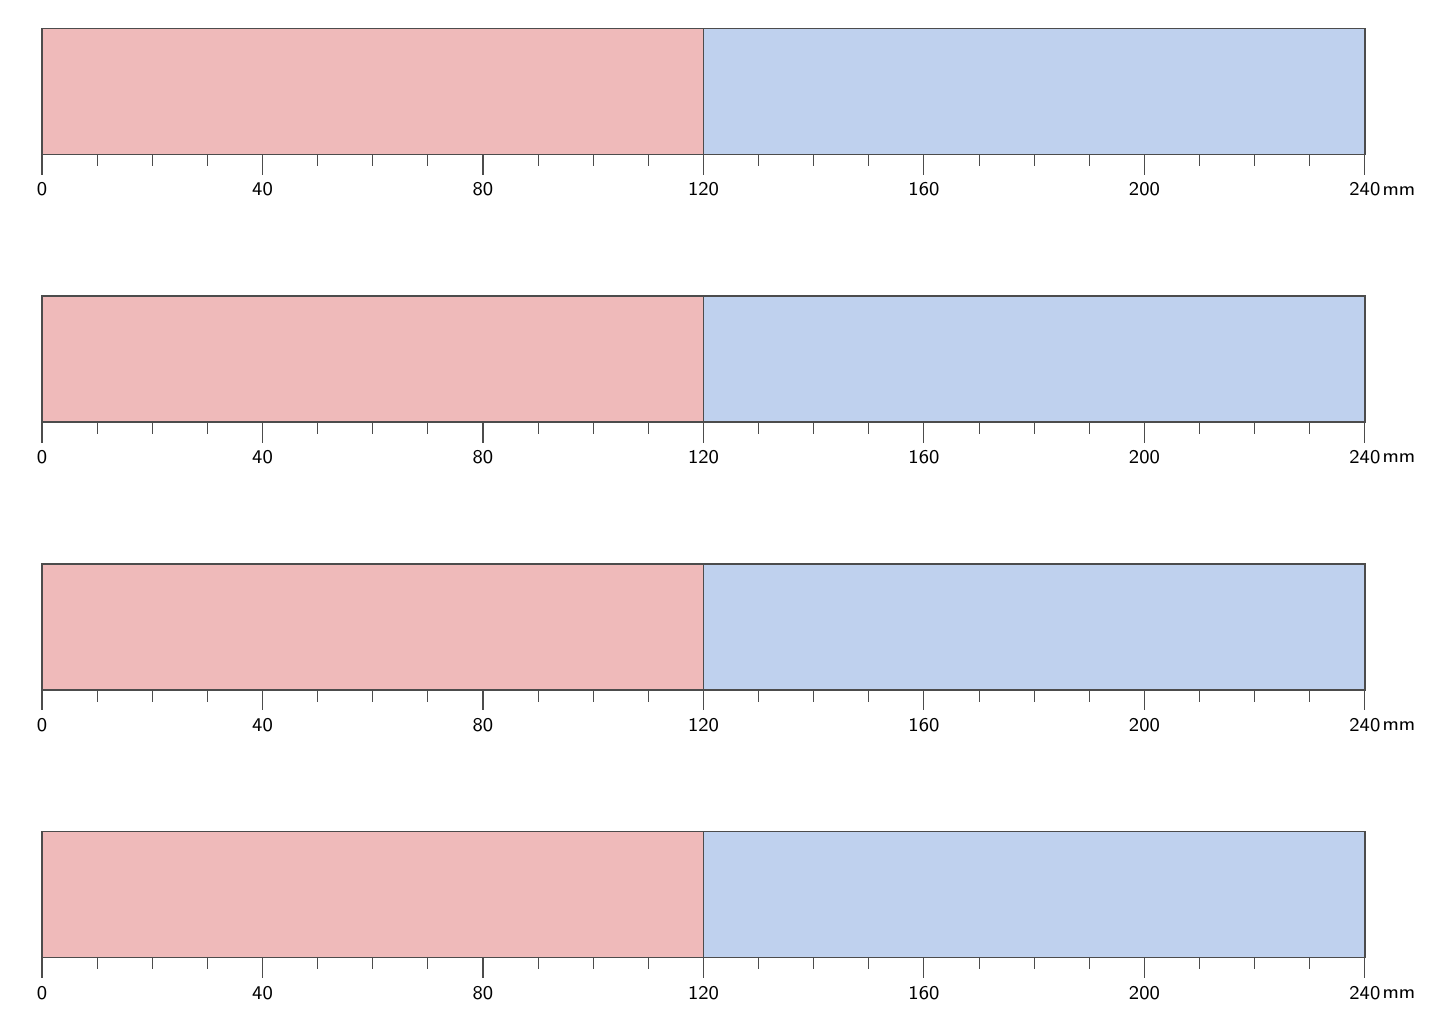
\begin{tikzpicture}[x=1mm,y=1mm]
\fill[stripred] (0,0) rectangle (84,16);
\fill[stripblue] (84,0) rectangle (168,16);
\draw[black!70, line width=0.6pt] (0,0) rectangle (168,16);
\draw[black!70, line width=0.6pt] (84,0) -- (84,16);
\draw[black!70, line width=0.4pt] (0,0) -- (0,-2.6);
\node[font=\scriptsize, below] at (0,-2.4) {0};
\draw[black!70, line width=0.4pt] (7,0) -- (7,-1.5);
\draw[black!70, line width=0.4pt] (14,0) -- (14,-1.5);
\draw[black!70, line width=0.4pt] (21,0) -- (21,-1.5);
\draw[black!70, line width=0.4pt] (28,0) -- (28,-2.6);
\node[font=\scriptsize, below] at (28,-2.4) {40};
\draw[black!70, line width=0.4pt] (35,0) -- (35,-1.5);
\draw[black!70, line width=0.4pt] (42,0) -- (42,-1.5);
\draw[black!70, line width=0.4pt] (49,0) -- (49,-1.5);
\draw[black!70, line width=0.4pt] (56,0) -- (56,-2.6);
\node[font=\scriptsize, below] at (56,-2.4) {80};
\draw[black!70, line width=0.4pt] (63,0) -- (63,-1.5);
\draw[black!70, line width=0.4pt] (70,0) -- (70,-1.5);
\draw[black!70, line width=0.4pt] (77,0) -- (77,-1.5);
\draw[black!70, line width=0.4pt] (84,0) -- (84,-2.6);
\node[font=\scriptsize, below] at (84,-2.4) {120};
\draw[black!70, line width=0.4pt] (91,0) -- (91,-1.5);
\draw[black!70, line width=0.4pt] (98,0) -- (98,-1.5);
\draw[black!70, line width=0.4pt] (105,0) -- (105,-1.5);
\draw[black!70, line width=0.4pt] (112,0) -- (112,-2.6);
\node[font=\scriptsize, below] at (112,-2.4) {160};
\draw[black!70, line width=0.4pt] (119,0) -- (119,-1.5);
\draw[black!70, line width=0.4pt] (126,0) -- (126,-1.5);
\draw[black!70, line width=0.4pt] (133,0) -- (133,-1.5);
\draw[black!70, line width=0.4pt] (140,0) -- (140,-2.6);
\node[font=\scriptsize, below] at (140,-2.4) {200};
\draw[black!70, line width=0.4pt] (147,0) -- (147,-1.5);
\draw[black!70, line width=0.4pt] (154,0) -- (154,-1.5);
\draw[black!70, line width=0.4pt] (161,0) -- (161,-1.5);
\draw[black!70, line width=0.4pt] (168,0) -- (168,-2.6);
\node[font=\scriptsize, below] at (168,-2.4) {240};
\node[font=\scriptsize, right] at (169,-4.6) {mm};
\fill[stripred] (0,-34) rectangle (84,-18);
\fill[stripblue] (84,-34) rectangle (168,-18);
\draw[black!70, line width=0.6pt] (0,-34) rectangle (168,-18);
\draw[black!70, line width=0.6pt] (84,-34) -- (84,-18);
\draw[black!70, line width=0.4pt] (0,-34) -- (0,-36.6);
\node[font=\scriptsize, below] at (0,-36.4) {0};
\draw[black!70, line width=0.4pt] (7,-34) -- (7,-35.5);
\draw[black!70, line width=0.4pt] (14,-34) -- (14,-35.5);
\draw[black!70, line width=0.4pt] (21,-34) -- (21,-35.5);
\draw[black!70, line width=0.4pt] (28,-34) -- (28,-36.6);
\node[font=\scriptsize, below] at (28,-36.4) {40};
\draw[black!70, line width=0.4pt] (35,-34) -- (35,-35.5);
\draw[black!70, line width=0.4pt] (42,-34) -- (42,-35.5);
\draw[black!70, line width=0.4pt] (49,-34) -- (49,-35.5);
\draw[black!70, line width=0.4pt] (56,-34) -- (56,-36.6);
\node[font=\scriptsize, below] at (56,-36.4) {80};
\draw[black!70, line width=0.4pt] (63,-34) -- (63,-35.5);
\draw[black!70, line width=0.4pt] (70,-34) -- (70,-35.5);
\draw[black!70, line width=0.4pt] (77,-34) -- (77,-35.5);
\draw[black!70, line width=0.4pt] (84,-34) -- (84,-36.6);
\node[font=\scriptsize, below] at (84,-36.4) {120};
\draw[black!70, line width=0.4pt] (91,-34) -- (91,-35.5);
\draw[black!70, line width=0.4pt] (98,-34) -- (98,-35.5);
\draw[black!70, line width=0.4pt] (105,-34) -- (105,-35.5);
\draw[black!70, line width=0.4pt] (112,-34) -- (112,-36.6);
\node[font=\scriptsize, below] at (112,-36.4) {160};
\draw[black!70, line width=0.4pt] (119,-34) -- (119,-35.5);
\draw[black!70, line width=0.4pt] (126,-34) -- (126,-35.5);
\draw[black!70, line width=0.4pt] (133,-34) -- (133,-35.5);
\draw[black!70, line width=0.4pt] (140,-34) -- (140,-36.6);
\node[font=\scriptsize, below] at (140,-36.4) {200};
\draw[black!70, line width=0.4pt] (147,-34) -- (147,-35.5);
\draw[black!70, line width=0.4pt] (154,-34) -- (154,-35.5);
\draw[black!70, line width=0.4pt] (161,-34) -- (161,-35.5);
\draw[black!70, line width=0.4pt] (168,-34) -- (168,-36.6);
\node[font=\scriptsize, below] at (168,-36.4) {240};
\node[font=\scriptsize, right] at (169,-38.6) {mm};
\fill[stripred] (0,-68) rectangle (84,-52);
\fill[stripblue] (84,-68) rectangle (168,-52);
\draw[black!70, line width=0.6pt] (0,-68) rectangle (168,-52);
\draw[black!70, line width=0.6pt] (84,-68) -- (84,-52);
\draw[black!70, line width=0.4pt] (0,-68) -- (0,-70.6);
\node[font=\scriptsize, below] at (0,-70.4) {0};
\draw[black!70, line width=0.4pt] (7,-68) -- (7,-69.5);
\draw[black!70, line width=0.4pt] (14,-68) -- (14,-69.5);
\draw[black!70, line width=0.4pt] (21,-68) -- (21,-69.5);
\draw[black!70, line width=0.4pt] (28,-68) -- (28,-70.6);
\node[font=\scriptsize, below] at (28,-70.4) {40};
\draw[black!70, line width=0.4pt] (35,-68) -- (35,-69.5);
\draw[black!70, line width=0.4pt] (42,-68) -- (42,-69.5);
\draw[black!70, line width=0.4pt] (49,-68) -- (49,-69.5);
\draw[black!70, line width=0.4pt] (56,-68) -- (56,-70.6);
\node[font=\scriptsize, below] at (56,-70.4) {80};
\draw[black!70, line width=0.4pt] (63,-68) -- (63,-69.5);
\draw[black!70, line width=0.4pt] (70,-68) -- (70,-69.5);
\draw[black!70, line width=0.4pt] (77,-68) -- (77,-69.5);
\draw[black!70, line width=0.4pt] (84,-68) -- (84,-70.6);
\node[font=\scriptsize, below] at (84,-70.4) {120};
\draw[black!70, line width=0.4pt] (91,-68) -- (91,-69.5);
\draw[black!70, line width=0.4pt] (98,-68) -- (98,-69.5);
\draw[black!70, line width=0.4pt] (105,-68) -- (105,-69.5);
\draw[black!70, line width=0.4pt] (112,-68) -- (112,-70.6);
\node[font=\scriptsize, below] at (112,-70.4) {160};
\draw[black!70, line width=0.4pt] (119,-68) -- (119,-69.5);
\draw[black!70, line width=0.4pt] (126,-68) -- (126,-69.5);
\draw[black!70, line width=0.4pt] (133,-68) -- (133,-69.5);
\draw[black!70, line width=0.4pt] (140,-68) -- (140,-70.6);
\node[font=\scriptsize, below] at (140,-70.4) {200};
\draw[black!70, line width=0.4pt] (147,-68) -- (147,-69.5);
\draw[black!70, line width=0.4pt] (154,-68) -- (154,-69.5);
\draw[black!70, line width=0.4pt] (161,-68) -- (161,-69.5);
\draw[black!70, line width=0.4pt] (168,-68) -- (168,-70.6);
\node[font=\scriptsize, below] at (168,-70.4) {240};
\node[font=\scriptsize, right] at (169,-72.6) {mm};
\fill[stripred] (0,-102) rectangle (84,-86);
\fill[stripblue] (84,-102) rectangle (168,-86);
\draw[black!70, line width=0.6pt] (0,-102) rectangle (168,-86);
\draw[black!70, line width=0.6pt] (84,-102) -- (84,-86);
\draw[black!70, line width=0.4pt] (0,-102) -- (0,-104.6);
\node[font=\scriptsize, below] at (0,-104.4) {0};
\draw[black!70, line width=0.4pt] (7,-102) -- (7,-103.5);
\draw[black!70, line width=0.4pt] (14,-102) -- (14,-103.5);
\draw[black!70, line width=0.4pt] (21,-102) -- (21,-103.5);
\draw[black!70, line width=0.4pt] (28,-102) -- (28,-104.6);
\node[font=\scriptsize, below] at (28,-104.4) {40};
\draw[black!70, line width=0.4pt] (35,-102) -- (35,-103.5);
\draw[black!70, line width=0.4pt] (42,-102) -- (42,-103.5);
\draw[black!70, line width=0.4pt] (49,-102) -- (49,-103.5);
\draw[black!70, line width=0.4pt] (56,-102) -- (56,-104.6);
\node[font=\scriptsize, below] at (56,-104.4) {80};
\draw[black!70, line width=0.4pt] (63,-102) -- (63,-103.5);
\draw[black!70, line width=0.4pt] (70,-102) -- (70,-103.5);
\draw[black!70, line width=0.4pt] (77,-102) -- (77,-103.5);
\draw[black!70, line width=0.4pt] (84,-102) -- (84,-104.6);
\node[font=\scriptsize, below] at (84,-104.4) {120};
\draw[black!70, line width=0.4pt] (91,-102) -- (91,-103.5);
\draw[black!70, line width=0.4pt] (98,-102) -- (98,-103.5);
\draw[black!70, line width=0.4pt] (105,-102) -- (105,-103.5);
\draw[black!70, line width=0.4pt] (112,-102) -- (112,-104.6);
\node[font=\scriptsize, below] at (112,-104.4) {160};
\draw[black!70, line width=0.4pt] (119,-102) -- (119,-103.5);
\draw[black!70, line width=0.4pt] (126,-102) -- (126,-103.5);
\draw[black!70, line width=0.4pt] (133,-102) -- (133,-103.5);
\draw[black!70, line width=0.4pt] (140,-102) -- (140,-104.6);
\node[font=\scriptsize, below] at (140,-104.4) {200};
\draw[black!70, line width=0.4pt] (147,-102) -- (147,-103.5);
\draw[black!70, line width=0.4pt] (154,-102) -- (154,-103.5);
\draw[black!70, line width=0.4pt] (161,-102) -- (161,-103.5);
\draw[black!70, line width=0.4pt] (168,-102) -- (168,-104.6);
\node[font=\scriptsize, below] at (168,-104.4) {240};
\node[font=\scriptsize, right] at (169,-106.6) {mm};
\end{tikzpicture}
\end{center}
\newpage
\prob{4}Can you make a train that needs three cuts to share it? Use an even number of red cards and an even number of blue cards.
\vspace{4mm}
\begin{center}

\begin{tikzpicture}[x=1mm,y=1mm]
\draw[boxgrey, line width=0.5pt, rounded corners=1.26mm] (0,0) rectangle (10.5,10.5);
\draw[boxgrey, line width=0.5pt, rounded corners=1.26mm] (15,0) rectangle (25.5,10.5);
\draw[boxgrey, line width=0.5pt, rounded corners=1.26mm] (30,0) rectangle (40.5,10.5);
\draw[boxgrey, line width=0.5pt, rounded corners=1.26mm] (45,0) rectangle (55.5,10.5);
\draw[boxgrey, line width=0.5pt, rounded corners=1.26mm] (60,0) rectangle (70.5,10.5);
\draw[boxgrey, line width=0.5pt, rounded corners=1.26mm] (75,0) rectangle (85.5,10.5);
\draw[boxgrey, line width=0.5pt, rounded corners=1.26mm] (90,0) rectangle (100.5,10.5);
\draw[boxgrey, line width=0.5pt, rounded corners=1.26mm] (105,0) rectangle (115.5,10.5);
\draw[boxgrey, line width=0.5pt, rounded corners=1.26mm] (120,0) rectangle (130.5,10.5);
\draw[boxgrey, line width=0.5pt, rounded corners=1.26mm] (135,0) rectangle (145.5,10.5);
\draw[boxgrey, line width=0.5pt, rounded corners=1.26mm] (150,0) rectangle (160.5,10.5);
\draw[boxgrey, line width=0.5pt, rounded corners=1.26mm] (165,0) rectangle (175.5,10.5);
\draw[boxgrey, line width=0.5pt, rounded corners=1.26mm] (0,-21) rectangle (10.5,-10.5);
\draw[boxgrey, line width=0.5pt, rounded corners=1.26mm] (15,-21) rectangle (25.5,-10.5);
\draw[boxgrey, line width=0.5pt, rounded corners=1.26mm] (30,-21) rectangle (40.5,-10.5);
\draw[boxgrey, line width=0.5pt, rounded corners=1.26mm] (45,-21) rectangle (55.5,-10.5);
\draw[boxgrey, line width=0.5pt, rounded corners=1.26mm] (60,-21) rectangle (70.5,-10.5);
\draw[boxgrey, line width=0.5pt, rounded corners=1.26mm] (75,-21) rectangle (85.5,-10.5);
\draw[boxgrey, line width=0.5pt, rounded corners=1.26mm] (90,-21) rectangle (100.5,-10.5);
\draw[boxgrey, line width=0.5pt, rounded corners=1.26mm] (105,-21) rectangle (115.5,-10.5);
\draw[boxgrey, line width=0.5pt, rounded corners=1.26mm] (120,-21) rectangle (130.5,-10.5);
\draw[boxgrey, line width=0.5pt, rounded corners=1.26mm] (135,-21) rectangle (145.5,-10.5);
\draw[boxgrey, line width=0.5pt, rounded corners=1.26mm] (150,-21) rectangle (160.5,-10.5);
\draw[boxgrey, line width=0.5pt, rounded corners=1.26mm] (165,-21) rectangle (175.5,-10.5);
\draw[boxgrey, line width=0.5pt, rounded corners=1.26mm] (0,-42) rectangle (10.5,-31.5);
\draw[boxgrey, line width=0.5pt, rounded corners=1.26mm] (15,-42) rectangle (25.5,-31.5);
\draw[boxgrey, line width=0.5pt, rounded corners=1.26mm] (30,-42) rectangle (40.5,-31.5);
\draw[boxgrey, line width=0.5pt, rounded corners=1.26mm] (45,-42) rectangle (55.5,-31.5);
\draw[boxgrey, line width=0.5pt, rounded corners=1.26mm] (60,-42) rectangle (70.5,-31.5);
\draw[boxgrey, line width=0.5pt, rounded corners=1.26mm] (75,-42) rectangle (85.5,-31.5);
\draw[boxgrey, line width=0.5pt, rounded corners=1.26mm] (90,-42) rectangle (100.5,-31.5);
\draw[boxgrey, line width=0.5pt, rounded corners=1.26mm] (105,-42) rectangle (115.5,-31.5);
\draw[boxgrey, line width=0.5pt, rounded corners=1.26mm] (120,-42) rectangle (130.5,-31.5);
\draw[boxgrey, line width=0.5pt, rounded corners=1.26mm] (135,-42) rectangle (145.5,-31.5);
\draw[boxgrey, line width=0.5pt, rounded corners=1.26mm] (150,-42) rectangle (160.5,-31.5);
\draw[boxgrey, line width=0.5pt, rounded corners=1.26mm] (165,-42) rectangle (175.5,-31.5);
\draw[boxgrey, line width=0.5pt, rounded corners=1.26mm] (0,-63) rectangle (10.5,-52.5);
\draw[boxgrey, line width=0.5pt, rounded corners=1.26mm] (15,-63) rectangle (25.5,-52.5);
\draw[boxgrey, line width=0.5pt, rounded corners=1.26mm] (30,-63) rectangle (40.5,-52.5);
\draw[boxgrey, line width=0.5pt, rounded corners=1.26mm] (45,-63) rectangle (55.5,-52.5);
\draw[boxgrey, line width=0.5pt, rounded corners=1.26mm] (60,-63) rectangle (70.5,-52.5);
\draw[boxgrey, line width=0.5pt, rounded corners=1.26mm] (75,-63) rectangle (85.5,-52.5);
\draw[boxgrey, line width=0.5pt, rounded corners=1.26mm] (90,-63) rectangle (100.5,-52.5);
\draw[boxgrey, line width=0.5pt, rounded corners=1.26mm] (105,-63) rectangle (115.5,-52.5);
\draw[boxgrey, line width=0.5pt, rounded corners=1.26mm] (120,-63) rectangle (130.5,-52.5);
\draw[boxgrey, line width=0.5pt, rounded corners=1.26mm] (135,-63) rectangle (145.5,-52.5);
\draw[boxgrey, line width=0.5pt, rounded corners=1.26mm] (150,-63) rectangle (160.5,-52.5);
\draw[boxgrey, line width=0.5pt, rounded corners=1.26mm] (165,-63) rectangle (175.5,-52.5);
\draw[boxgrey, line width=0.5pt, rounded corners=1.26mm] (0,-84) rectangle (10.5,-73.5);
\draw[boxgrey, line width=0.5pt, rounded corners=1.26mm] (15,-84) rectangle (25.5,-73.5);
\draw[boxgrey, line width=0.5pt, rounded corners=1.26mm] (30,-84) rectangle (40.5,-73.5);
\draw[boxgrey, line width=0.5pt, rounded corners=1.26mm] (45,-84) rectangle (55.5,-73.5);
\draw[boxgrey, line width=0.5pt, rounded corners=1.26mm] (60,-84) rectangle (70.5,-73.5);
\draw[boxgrey, line width=0.5pt, rounded corners=1.26mm] (75,-84) rectangle (85.5,-73.5);
\draw[boxgrey, line width=0.5pt, rounded corners=1.26mm] (90,-84) rectangle (100.5,-73.5);
\draw[boxgrey, line width=0.5pt, rounded corners=1.26mm] (105,-84) rectangle (115.5,-73.5);
\draw[boxgrey, line width=0.5pt, rounded corners=1.26mm] (120,-84) rectangle (130.5,-73.5);
\draw[boxgrey, line width=0.5pt, rounded corners=1.26mm] (135,-84) rectangle (145.5,-73.5);
\draw[boxgrey, line width=0.5pt, rounded corners=1.26mm] (150,-84) rectangle (160.5,-73.5);
\draw[boxgrey, line width=0.5pt, rounded corners=1.26mm] (165,-84) rectangle (175.5,-73.5);
\draw[boxgrey, line width=0.5pt, rounded corners=1.26mm] (0,-105) rectangle (10.5,-94.5);
\draw[boxgrey, line width=0.5pt, rounded corners=1.26mm] (15,-105) rectangle (25.5,-94.5);
\draw[boxgrey, line width=0.5pt, rounded corners=1.26mm] (30,-105) rectangle (40.5,-94.5);
\draw[boxgrey, line width=0.5pt, rounded corners=1.26mm] (45,-105) rectangle (55.5,-94.5);
\draw[boxgrey, line width=0.5pt, rounded corners=1.26mm] (60,-105) rectangle (70.5,-94.5);
\draw[boxgrey, line width=0.5pt, rounded corners=1.26mm] (75,-105) rectangle (85.5,-94.5);
\draw[boxgrey, line width=0.5pt, rounded corners=1.26mm] (90,-105) rectangle (100.5,-94.5);
\draw[boxgrey, line width=0.5pt, rounded corners=1.26mm] (105,-105) rectangle (115.5,-94.5);
\draw[boxgrey, line width=0.5pt, rounded corners=1.26mm] (120,-105) rectangle (130.5,-94.5);
\draw[boxgrey, line width=0.5pt, rounded corners=1.26mm] (135,-105) rectangle (145.5,-94.5);
\draw[boxgrey, line width=0.5pt, rounded corners=1.26mm] (150,-105) rectangle (160.5,-94.5);
\draw[boxgrey, line width=0.5pt, rounded corners=1.26mm] (165,-105) rectangle (175.5,-94.5);
\draw[boxgrey, line width=0.5pt, rounded corners=1.26mm] (0,-126) rectangle (10.5,-115.5);
\draw[boxgrey, line width=0.5pt, rounded corners=1.26mm] (15,-126) rectangle (25.5,-115.5);
\draw[boxgrey, line width=0.5pt, rounded corners=1.26mm] (30,-126) rectangle (40.5,-115.5);
\draw[boxgrey, line width=0.5pt, rounded corners=1.26mm] (45,-126) rectangle (55.5,-115.5);
\draw[boxgrey, line width=0.5pt, rounded corners=1.26mm] (60,-126) rectangle (70.5,-115.5);
\draw[boxgrey, line width=0.5pt, rounded corners=1.26mm] (75,-126) rectangle (85.5,-115.5);
\draw[boxgrey, line width=0.5pt, rounded corners=1.26mm] (90,-126) rectangle (100.5,-115.5);
\draw[boxgrey, line width=0.5pt, rounded corners=1.26mm] (105,-126) rectangle (115.5,-115.5);
\draw[boxgrey, line width=0.5pt, rounded corners=1.26mm] (120,-126) rectangle (130.5,-115.5);
\draw[boxgrey, line width=0.5pt, rounded corners=1.26mm] (135,-126) rectangle (145.5,-115.5);
\draw[boxgrey, line width=0.5pt, rounded corners=1.26mm] (150,-126) rectangle (160.5,-115.5);
\draw[boxgrey, line width=0.5pt, rounded corners=1.26mm] (165,-126) rectangle (175.5,-115.5);
\draw[boxgrey, line width=0.5pt, rounded corners=1.26mm] (0,-147) rectangle (10.5,-136.5);
\draw[boxgrey, line width=0.5pt, rounded corners=1.26mm] (15,-147) rectangle (25.5,-136.5);
\draw[boxgrey, line width=0.5pt, rounded corners=1.26mm] (30,-147) rectangle (40.5,-136.5);
\draw[boxgrey, line width=0.5pt, rounded corners=1.26mm] (45,-147) rectangle (55.5,-136.5);
\draw[boxgrey, line width=0.5pt, rounded corners=1.26mm] (60,-147) rectangle (70.5,-136.5);
\draw[boxgrey, line width=0.5pt, rounded corners=1.26mm] (75,-147) rectangle (85.5,-136.5);
\draw[boxgrey, line width=0.5pt, rounded corners=1.26mm] (90,-147) rectangle (100.5,-136.5);
\draw[boxgrey, line width=0.5pt, rounded corners=1.26mm] (105,-147) rectangle (115.5,-136.5);
\draw[boxgrey, line width=0.5pt, rounded corners=1.26mm] (120,-147) rectangle (130.5,-136.5);
\draw[boxgrey, line width=0.5pt, rounded corners=1.26mm] (135,-147) rectangle (145.5,-136.5);
\draw[boxgrey, line width=0.5pt, rounded corners=1.26mm] (150,-147) rectangle (160.5,-136.5);
\draw[boxgrey, line width=0.5pt, rounded corners=1.26mm] (165,-147) rectangle (175.5,-136.5);
\end{tikzpicture}
\end{center}
\newpage
\prob{5}Three people use the three-person cards A, B and C, which give these values to the grey panels X, Y and Z.
\begin{center}
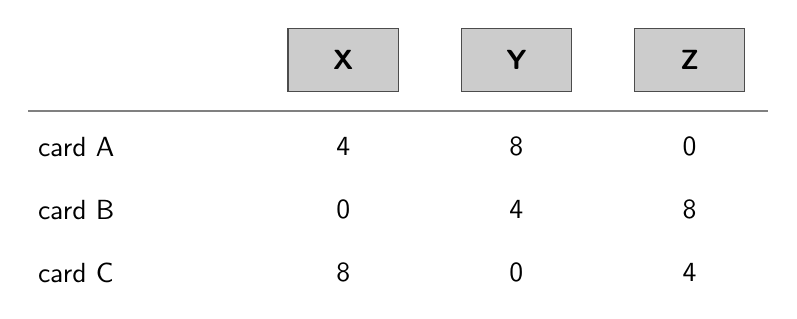
\begin{tikzpicture}[x=1mm,y=1mm]
\draw[black!70, fill=panelgrey, line width=0.5pt] (33,-8) rectangle (47,0);
\node[font=\bfseries] at (40,-4) {X};
\draw[black!70, fill=panelgrey, line width=0.5pt] (55,-8) rectangle (69,0);
\node[font=\bfseries] at (62,-4) {Y};
\draw[black!70, fill=panelgrey, line width=0.5pt] (77,-8) rectangle (91,0);
\node[font=\bfseries] at (84,-4) {Z};
\node[anchor=west] at (0,-15) {card A};
\node at (40,-15) {4};
\node at (62,-15) {8};
\node at (84,-15) {0};
\node[anchor=west] at (0,-23) {card B};
\node at (40,-23) {0};
\node at (62,-23) {4};
\node at (84,-23) {8};
\node[anchor=west] at (0,-31) {card C};
\node at (40,-31) {8};
\node at (62,-31) {0};
\node at (84,-31) {4};
\draw[black!50, line width=0.4pt] (0,-10.5) -- (94,-10.5);
\end{tikzpicture}
\end{center}
Each number is the value of a whole 50\,mm panel. A panel may be cut straight across, and value follows length within a panel:
\begin{center}
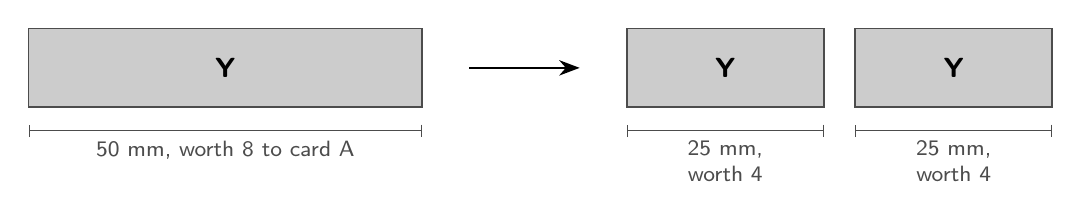
\begin{tikzpicture}[x=1mm,y=1mm]
\draw[black!70, fill=panelgrey, line width=0.6pt] (0,0) rectangle (50,10);
\node[font=\bfseries] at (25,5) {Y};
\draw[|-|, black!70, line width=0.4pt] (0,-3) -- node[below, font=\footnotesize] {50 mm, worth 8 to card A} (50,-3);
\draw[-{Stealth[length=2.6mm]}, line width=0.9pt] (56,5) -- (70,5);
\draw[black!70, fill=panelgrey, line width=0.6pt] (76,0) rectangle (101,10);
\node[font=\bfseries] at (88.5,5) {Y};
\draw[|-|, black!70, line width=0.4pt] (76,-3) -- node[below, font=\footnotesize, align=center] {25 mm,\\ worth 4} (101,-3);
\draw[black!70, fill=panelgrey, line width=0.6pt] (105,0) rectangle (130,10);
\node[font=\bfseries] at (117.5,5) {Y};
\draw[|-|, black!70, line width=0.4pt] (105,-3) -- node[below, font=\footnotesize, align=center] {25 mm,\\ worth 4} (130,-3);
\end{tikzpicture}
\end{center}
The three people share a row of the panels with a marking game, run by a referee. Each person marks where the piece from the left end first becomes worth 4 by their own card. Whoever marked leftmost takes that piece. The other two mark again from the new left end, aiming at 4 again, and whoever marked leftmost takes that piece. The last person takes the rest.
\begin{center}
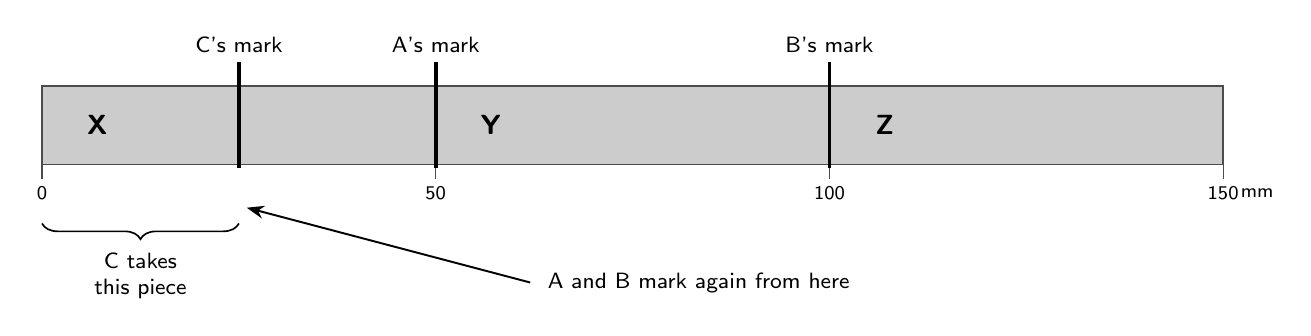
\begin{tikzpicture}[x=1mm,y=1mm]
\draw[black!70, fill=panelgrey, line width=0.6pt] (0,0) rectangle (50,10);
\node[font=\bfseries] at (7,5) {X};
\draw[black!70, fill=panelgrey, line width=0.6pt] (50,0) rectangle (100,10);
\node[font=\bfseries] at (57,5) {Y};
\draw[black!70, fill=panelgrey, line width=0.6pt] (100,0) rectangle (150,10);
\node[font=\bfseries] at (107,5) {Z};
\draw[black!70, line width=0.4pt] (0,0) -- (0,-1.8);
\node[font=\scriptsize, below] at (0,-1.6) {0};
\draw[black!70, line width=0.4pt] (50,0) -- (50,-1.8);
\node[font=\scriptsize, below] at (50,-1.6) {50};
\draw[black!70, line width=0.4pt] (100,0) -- (100,-1.8);
\node[font=\scriptsize, below] at (100,-1.6) {100};
\draw[black!70, line width=0.4pt] (150,0) -- (150,-1.8);
\node[font=\scriptsize, below] at (150,-1.6) {150};
\node[font=\scriptsize, right] at (151,-3.6) {mm};
\draw[black, line width=1.3pt] (25,-0.5) -- (25,13);
\node[font=\footnotesize, above] at (25,13) {C's mark};
\draw[black, line width=1.3pt] (50,-0.5) -- (50,13);
\node[font=\footnotesize, above] at (50,13) {A's mark};
\draw[black, line width=1.3pt] (100,-0.5) -- (100,13);
\node[font=\footnotesize, above] at (100,13) {B's mark};
\draw[decorate, decoration={brace, amplitude=2mm, mirror}, line width=0.6pt] (0,-7.5) -- (25,-7.5);
\node[font=\footnotesize, align=center, below] at (12.5,-10) {C takes\\this piece};
\draw[-{Stealth[length=2.2mm]}, line width=0.7pt] (62,-15) -- (26,-5.5);
\node[font=\footnotesize, anchor=west] at (63,-15) {A and B mark again from here};
\end{tikzpicture}
\end{center}
Play the game with the panels in the order X~Z~Y.
\vspace{3mm}
\begin{center}
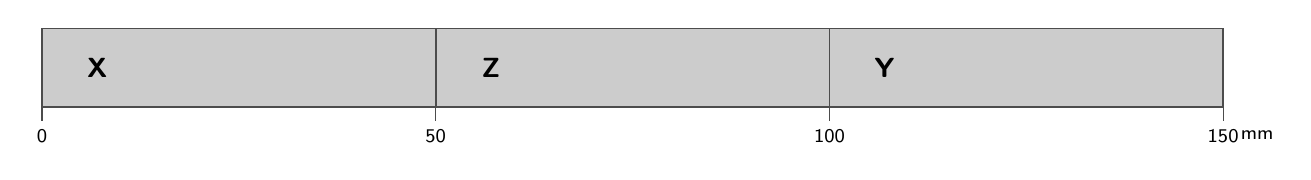
\begin{tikzpicture}[x=1mm,y=1mm]
\draw[black!70, fill=panelgrey, line width=0.6pt] (0,0) rectangle (50,10);
\node[font=\bfseries] at (7,5) {X};
\draw[black!70, fill=panelgrey, line width=0.6pt] (50,0) rectangle (100,10);
\node[font=\bfseries] at (57,5) {Z};
\draw[black!70, fill=panelgrey, line width=0.6pt] (100,0) rectangle (150,10);
\node[font=\bfseries] at (107,5) {Y};
\draw[black!70, line width=0.4pt] (0,0) -- (0,-1.8);
\node[font=\scriptsize, below] at (0,-1.6) {0};
\draw[black!70, line width=0.4pt] (50,0) -- (50,-1.8);
\node[font=\scriptsize, below] at (50,-1.6) {50};
\draw[black!70, line width=0.4pt] (100,0) -- (100,-1.8);
\node[font=\scriptsize, below] at (100,-1.6) {100};
\draw[black!70, line width=0.4pt] (150,0) -- (150,-1.8);
\node[font=\scriptsize, below] at (150,-1.6) {150};
\node[font=\scriptsize, right] at (151,-3.6) {mm};
\end{tikzpicture}
\end{center}
\newpage
\prob{6}Play the game again with the panels in the orders Y~X~Z and Z~Y~X. In your three games, does anyone get less than 4 by their own card? Would anyone rather have someone else's piece?
\vspace{6mm}
\begin{center}
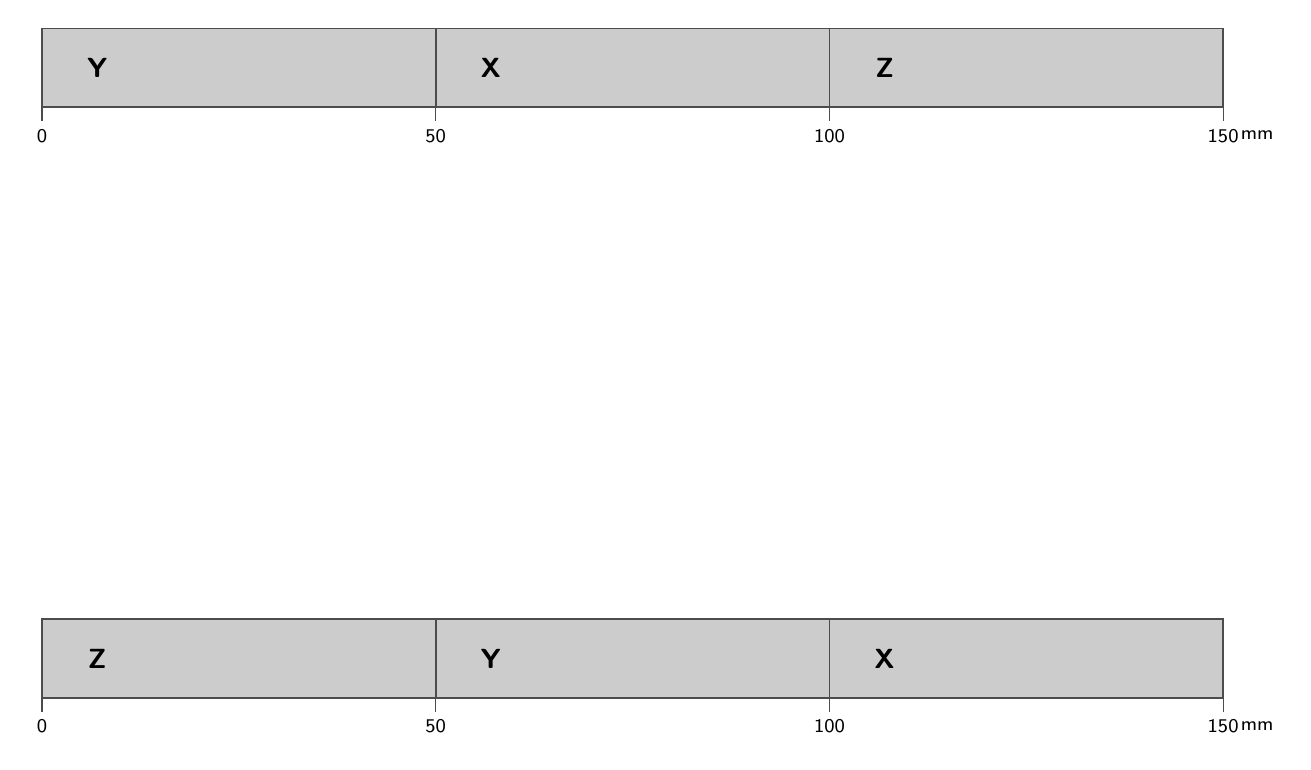
\begin{tikzpicture}[x=1mm,y=1mm]
\draw[black!70, fill=panelgrey, line width=0.6pt] (0,0) rectangle (50,10);
\node[font=\bfseries] at (7,5) {Y};
\draw[black!70, fill=panelgrey, line width=0.6pt] (50,0) rectangle (100,10);
\node[font=\bfseries] at (57,5) {X};
\draw[black!70, fill=panelgrey, line width=0.6pt] (100,0) rectangle (150,10);
\node[font=\bfseries] at (107,5) {Z};
\draw[black!70, line width=0.4pt] (0,0) -- (0,-1.8);
\node[font=\scriptsize, below] at (0,-1.6) {0};
\draw[black!70, line width=0.4pt] (50,0) -- (50,-1.8);
\node[font=\scriptsize, below] at (50,-1.6) {50};
\draw[black!70, line width=0.4pt] (100,0) -- (100,-1.8);
\node[font=\scriptsize, below] at (100,-1.6) {100};
\draw[black!70, line width=0.4pt] (150,0) -- (150,-1.8);
\node[font=\scriptsize, below] at (150,-1.6) {150};
\node[font=\scriptsize, right] at (151,-3.6) {mm};
\draw[black!70, fill=panelgrey, line width=0.6pt] (0,-75) rectangle (50,-65);
\node[font=\bfseries] at (7,-70) {Z};
\draw[black!70, fill=panelgrey, line width=0.6pt] (50,-75) rectangle (100,-65);
\node[font=\bfseries] at (57,-70) {Y};
\draw[black!70, fill=panelgrey, line width=0.6pt] (100,-75) rectangle (150,-65);
\node[font=\bfseries] at (107,-70) {X};
\draw[black!70, line width=0.4pt] (0,-75) -- (0,-76.8);
\node[font=\scriptsize, below] at (0,-76.6) {0};
\draw[black!70, line width=0.4pt] (50,-75) -- (50,-76.8);
\node[font=\scriptsize, below] at (50,-76.6) {50};
\draw[black!70, line width=0.4pt] (100,-75) -- (100,-76.8);
\node[font=\scriptsize, below] at (100,-76.6) {100};
\draw[black!70, line width=0.4pt] (150,-75) -- (150,-76.8);
\node[font=\scriptsize, below] at (150,-76.6) {150};
\node[font=\scriptsize, right] at (151,-78.6) {mm};
\end{tikzpicture}
\end{center}

\end{document}
